
In the past experiments we calibrated the measurement pulses and the drive pulses so, at this point, what is missing from a basic calibration point of view is just the states classification~\cite{Caban2015, Dietrich2022}.

The experiment is very easy, but can still be fine-tuned for readout calibration.
The procedure is at follows:
\begin{itemize}
    \item we prepare the qubit in state $\ket 0$ (waiting enough time) and we measure \textit{without} averaging;
    \item we prepare the qubit in state $\ket 1$ (applying a \pipulse) and we measure \textit{without} averaging;
    \item we repeat the experiment and we plot in the IQ plane the single shots.
\end{itemize}

In \cref{fig:sketch_single_shot_class} an ideal sketch-plot for the experiment is presented.

\begin{figure}[ht]
    \centering
    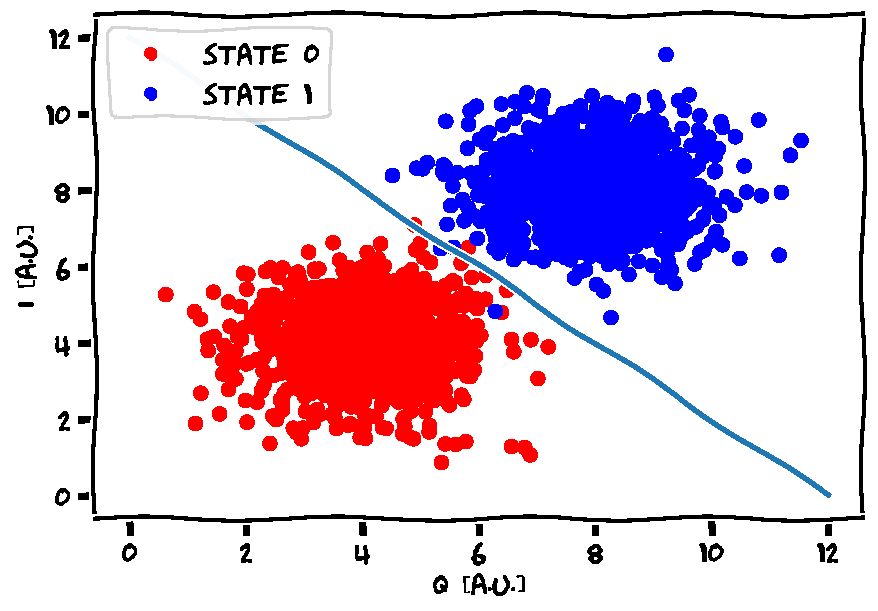
\includegraphics[width=0.5\textwidth]{characterization/figures/classification_sketch.pdf}
    \caption{Ideal plot for a single-shot classification experiment.}
    \label{fig:sketch_single_shot_class}
\end{figure}

The task now is to define a classification scheme that enables to assign a state (0-1) to every point in the IQ plane. 
Different scheme more or less efficient can be employed (based on Machine Learning, ...) but usually the definition of a simple straight division line is enough.
To find it, we proceed as follows:
\begin{itemize}
    \item we find the mean points for state 0 and 1;
    \item we perform a rotation of the angle identified by the segment between the two mean points. Namely, we rotate the IQ plane so that the two mean points are on the same horizontal line;
    \item we focus on the real parts and perform the cumulative distribution of the points of state 0 and state 1 (considering all the points);
    \item we compute the difference point-by-point between the two cumulative distributions and select as threshold the value that maximize this difference.
\end{itemize}

In this way we are maximizing, with a single straight line, the \textit{assignment fidelity} defined as:
\begin{equation}
    \text{assignment fidelity} = \frac{\text{correct predictions}}{\text{total number of points}}
\end{equation}
The two parameters that we have to save to use them in later experiments and circuit executions are the rotation angle and the threshold~\footnote{Note that we can consider these two parameter sufficiently stable, but still this experiment needs to be executed every now and then even in ideal cases. Moreover, for RFSoCs systems, the rotation angle can change every time the firmware is re-loaded into the FPGA logic.}.

The assignment fidelity is the first single number that describes the "goodness" of the qubit and its calibration. 
For the qubit to work in the best way, this number should be higher than 90-95\% but note that the real fidelity number (namely gate-fidelity) will be computed with a different experiment.

\begin{figure}[ht]
    \centering
    \subfloat[\centering Assignment fidelity = $0.80$]{
        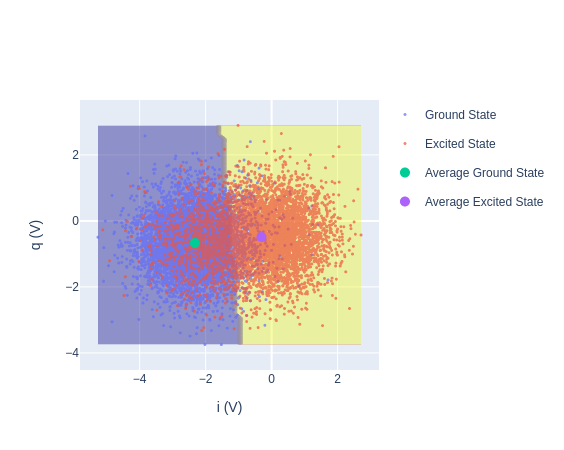
\includegraphics[width=0.6\textwidth]{characterization/figures/single_shot_80.png}
    }\\
    \subfloat[\centering Assignment fidelity = $0.92$]{
        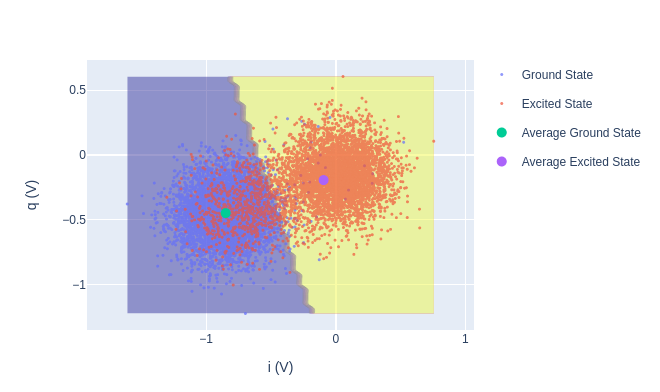
\includegraphics[width=0.6\textwidth]{characterization/figures/classification_92.png}
    }
    \caption{At the top, a possible bad plot in a single-shot classification experiment. At the bottom, a good one.}%
    \label{fig:single_shot_class_80_60}
\end{figure}


In real case scenario, sadly too often, the classification plot can look as \cref{fig:single_shot_class_80_60}(a).
The problem can be something hardware related, caused to the qubit fabrication and inherent S/N ratio so cannot be improved arbitrarily, or fixable with a good calibration.
In particular, a longer measurement pulse can help to distance the two "blobs" in the IQ plane and also an increased measurement amplitude can improve the S/N leading to the same effect.
If the fidelity is still very low, a good hardware solution is to add a quantum limited amplifier (TWPA or JPA) to the readout line inside the cryostate.\\
In any case, the fact that the single shot fidelity is not great can be partially reduced as a problem by increasing the number of shots to execute whatever circuit of future experiment.

On the other hand, sometimes the calibration and qubit quality is enough to obtain a nice fidelity as in the bottom plot of \cref{fig:single_shot_class_80_60}.


%\begin{figure}[ht]
%    \centering
%    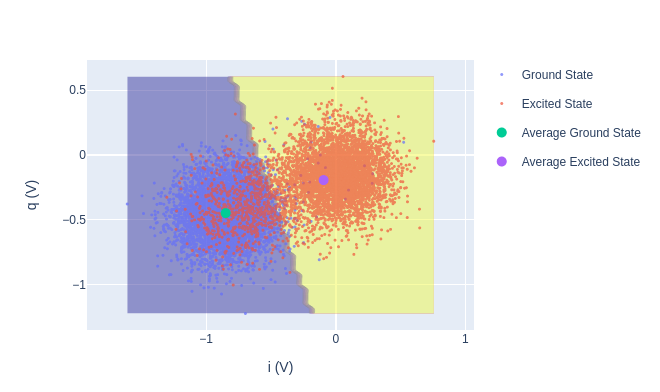
\includegraphics[width=0.9\textwidth]{characterization/figures/classification_92.png}
%    \caption{Good plot for a single-shot classification experiment (assignment fidelity of 0.92).}
%    \label{fig:single_shot_class}
%\end{figure}


\experimentrecap
{Single-shot classification}
{qubit characterization}
{threshold and rotation angle for classification,\\assignment fidelity}
{we prepare the qubit in the state zero and we measure the IQ values without averaging. We then prepare the qubit in state one and measure. We repeat the measurements a high number of times and we plot the the non-averaged results. We find the separation line that maximize the assignment fidelity, namely the fraction of right assignments}